\documentclass[tikz,border=10pt]{standalone}
\usepackage{amsmath}
\begin{document}

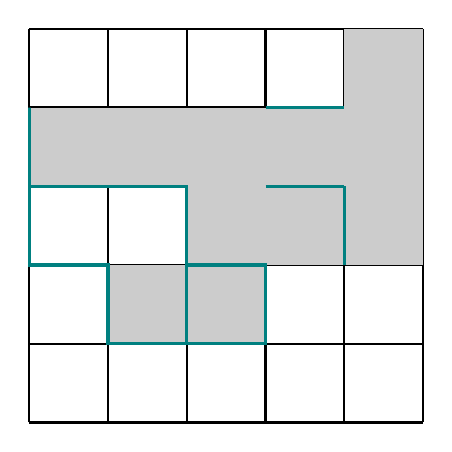
\begin{tikzpicture}
    % Define colors
    \definecolor{graycell}{rgb}{0.8,0.8,0.8}
    \definecolor{tealborder}{rgb}{0,0.5,0.5}
    
    % Draw the grid
    \draw[step=1cm, black, thick] (0,0) grid (5,5);

    % Fill the gray cells
    \foreach \x/\y in {0/3, 1/3, 2/3, 3/3, 3/2, 4/2, 4/3, 4/4, 1/1, 2/1, 2/2} {
        \fill[graycell] (\x,\y) rectangle ++(1,1);
    }

    % Highlight the perimeter with teal color
    \draw[tealborder, very thick] (0,4) -- (0,3) -- (2,3) -- (2,2) -- (3,2) -- (3,1) -- (1,1) -- (1,2) -- (0,2) -- cycle;
    \draw[tealborder, very thick] (2,2) -- (2,1);
    \draw[tealborder, very thick] (3,3) -- (4,3);
    \draw[tealborder, very thick] (4,2) -- (4,3);
    \draw[tealborder, very thick] (3,4) -- (4,4);

\end{tikzpicture}

\end{document}